\documentclass[12pt]{article}
\usepackage{braket}
\usepackage{physics}
\usepackage{graphicx}
\usepackage{times}
\usepackage[export]{adjustbox}
\usepackage{listings}
\usepackage{mathcomp}
\usepackage{hyperref}
\usepackage{bm,amsmath}
\usepackage{float}
\usepackage{indentfirst}
\usepackage{bigints}
\usepackage{listings}
\usepackage{color}
\hypersetup{
colorlinks=true,
linkcolor=blue,
filecolor=magenta,
urlcolor=cyan,
pdftitle={Overleaf Example},
pdfpagemode=FullScreen,
}
\definecolor{dkgreen}{rgb}{0,0.6,0}
\definecolor{gray}{rgb}{0.5,0.5,0.5}
\definecolor{mauve}{rgb}{0.58,0,0.82}
\lstset{frame=tb,
language=Python,
aboveskip=3mm,
belowskip=3mm,
stepnumber = 1,
showstringspaces=false,
columns=flexible,
basicstyle={\small\ttfamily},
numbers=left,
numberstyle=\color{gray},
keywordstyle=\color{blue},
commentstyle=\color{dkgreen},
stringstyle=\color{mauve},
breaklines=true,
breakatwhitespace=true,
tabsize=3
}
\numberwithin{equation}{section}

\title{Report on Particle Transformer for B-meson Decay}
\author{Ting-Kai Hsu}
\date{\today}

\begin{document}
\maketitle
\tableofcontents
\section{Regression but not Classification!}
The original design of Particle Transformer is for jet tagging, in ML language, is a classification CNN network.
One must change the model configuration into regression if we would like to reconstruct the B-meson decay.
First, the information of model in each train is stored in logs directory, which is very helpful for debugging.
There are few things to do with the code of the model and also some parameters need to be modified according.
\begin{itemize}
    \item Loss function: Cross entropy loss function is used for classification, meanwhile we should use MSE loss function for regression.
    \item Activation function: With the same reason as loss function, the activation function we should use in the output layer should be linear activation function rather than softmax.
    \item Dropout: The dropout layer could be 1 or 0, depends on whether you think the model would be overfitting or not.
\end{itemize}
\subsection{Questions for other unchanged parameters in model config}
However, I have some questions to ask.

First, what does dropout activation layer mean?
I used to have 1 activation dropout layer, and it ruins all the prediction output.

Second, what is the dynamics axes in the model configuration?

\subsection{Training Parameter}
Using 1 epoch can shorten the time for training, and changing the sample rate for training and validation would also shorten the processing time.
The default batch size of the model is 256, which is too big for my PC GPU, so I turn it to be 128.
\textbf{Important!} Please remember to turn on the regression mode by adding corresponding prefix when training.

\section{Results}
Result of 1 epoch, without dropout layer,
\begin{figure}[H]
    \centering
    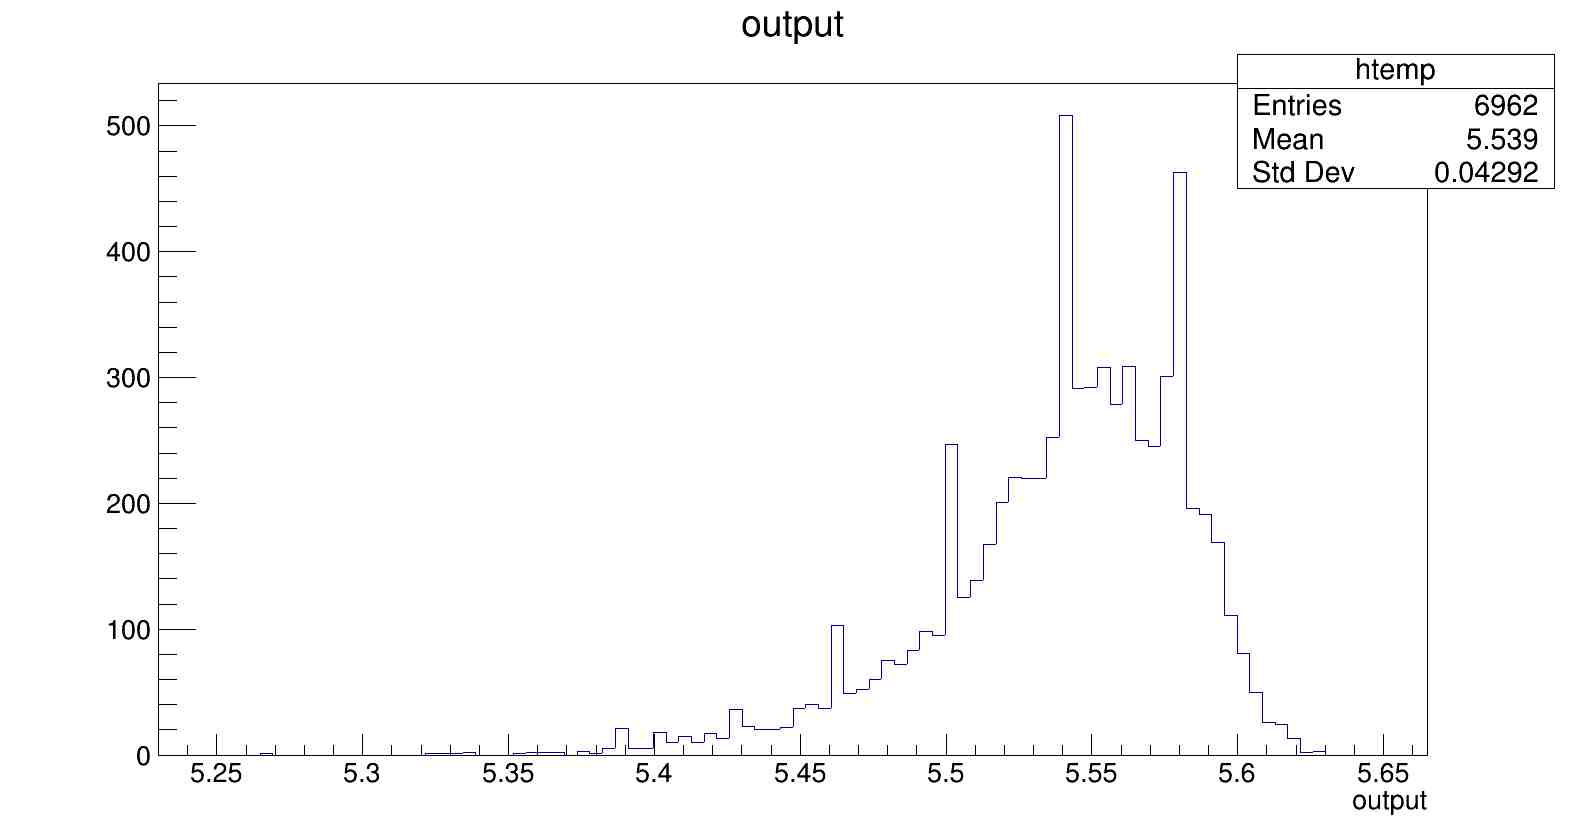
\includegraphics[width=0.75\linewidth]{figures/prediction.jpg}
    \caption{Prediction of 1 epoch without dropout layer}
    \label{}
\end{figure}
Result of 20 epochs, with 1 dropout layer,
\begin{figure}[H]
    \centering
    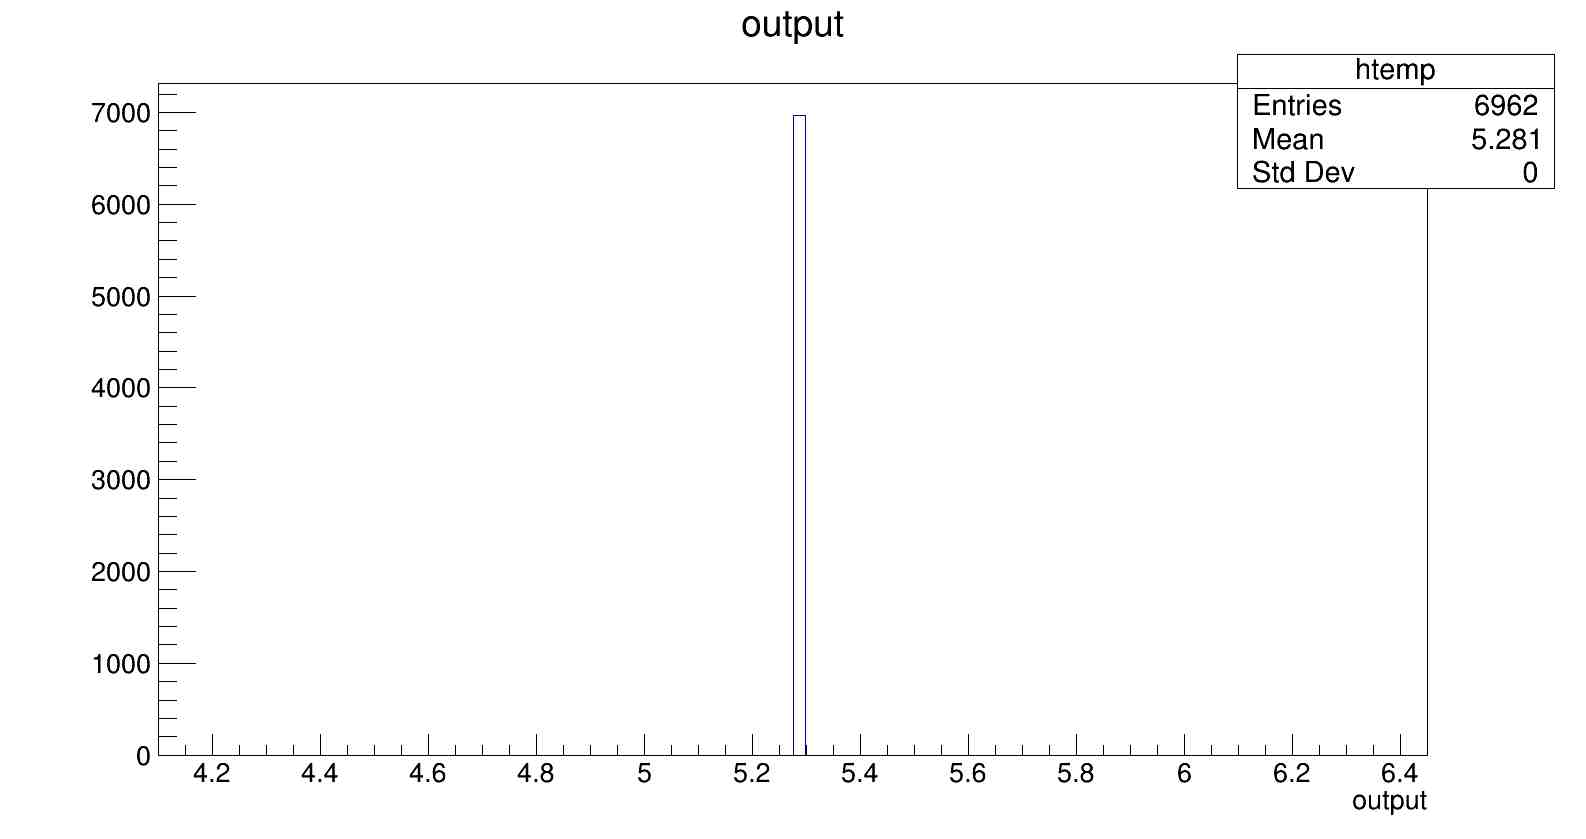
\includegraphics[width=0.75\linewidth]{figures/prediction20epochs.jpg}
    \caption{Prediction of 20 epochs with Dropout layer}
    \label{}
\end{figure}

\section{Fixing DividedByZero Error}
I change the precision of data from \textbf{float32} to \textbf{float64}, and this would at least decrease the probabilities of having zero in the data.

\section{New Result: Brief Comparison of Particle Net and Particle Transformer}
I run the training model first with standard configuration, and then find out the results are unsatisfied.
Then, I downgrade the batch size, the learning rate, and increase the validation per epoch and the number of epoches.

\begin{figure}[H]
    \centering
    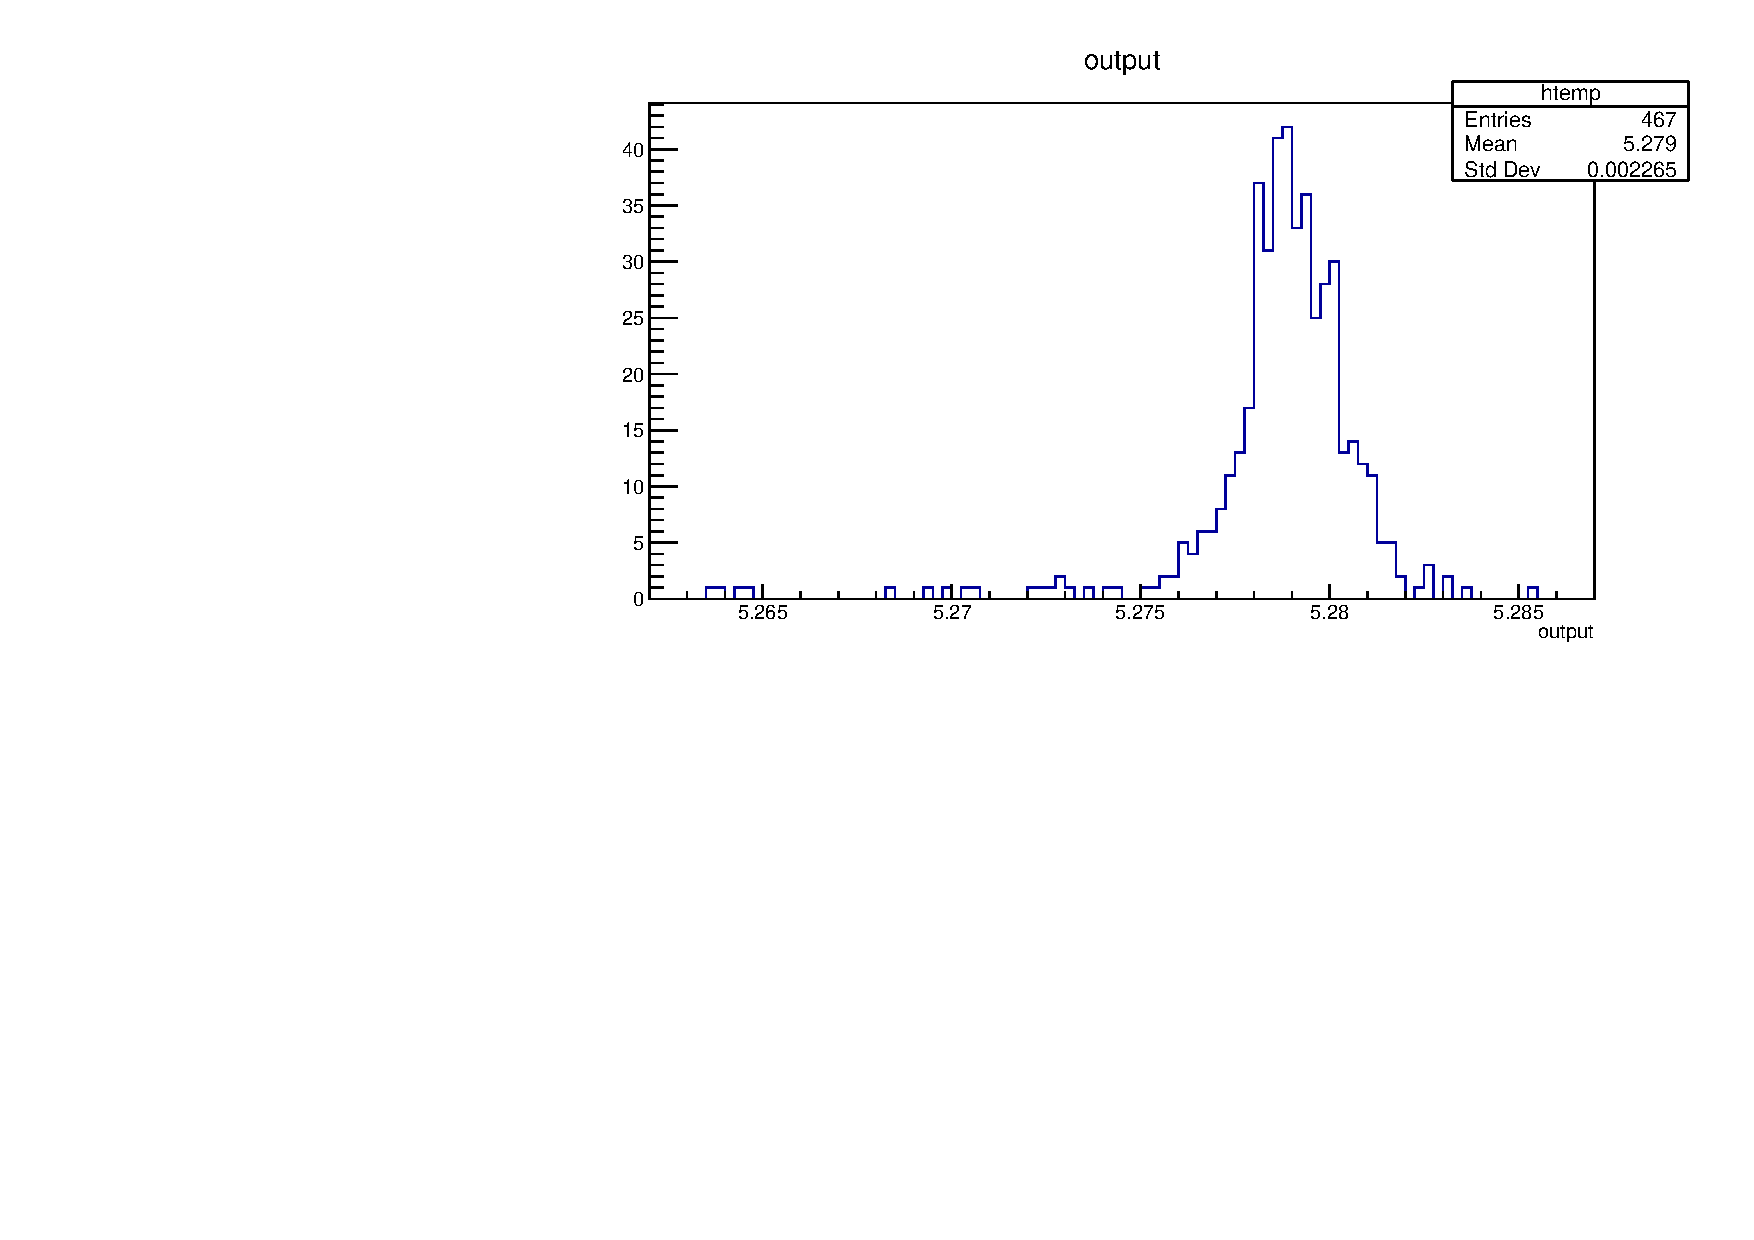
\includegraphics[width=0.5\linewidth]{figures/predPN1.pdf}
    \caption{PN1}
    \label{PN1}
\end{figure}
\begin{figure}[H]
    \centering
    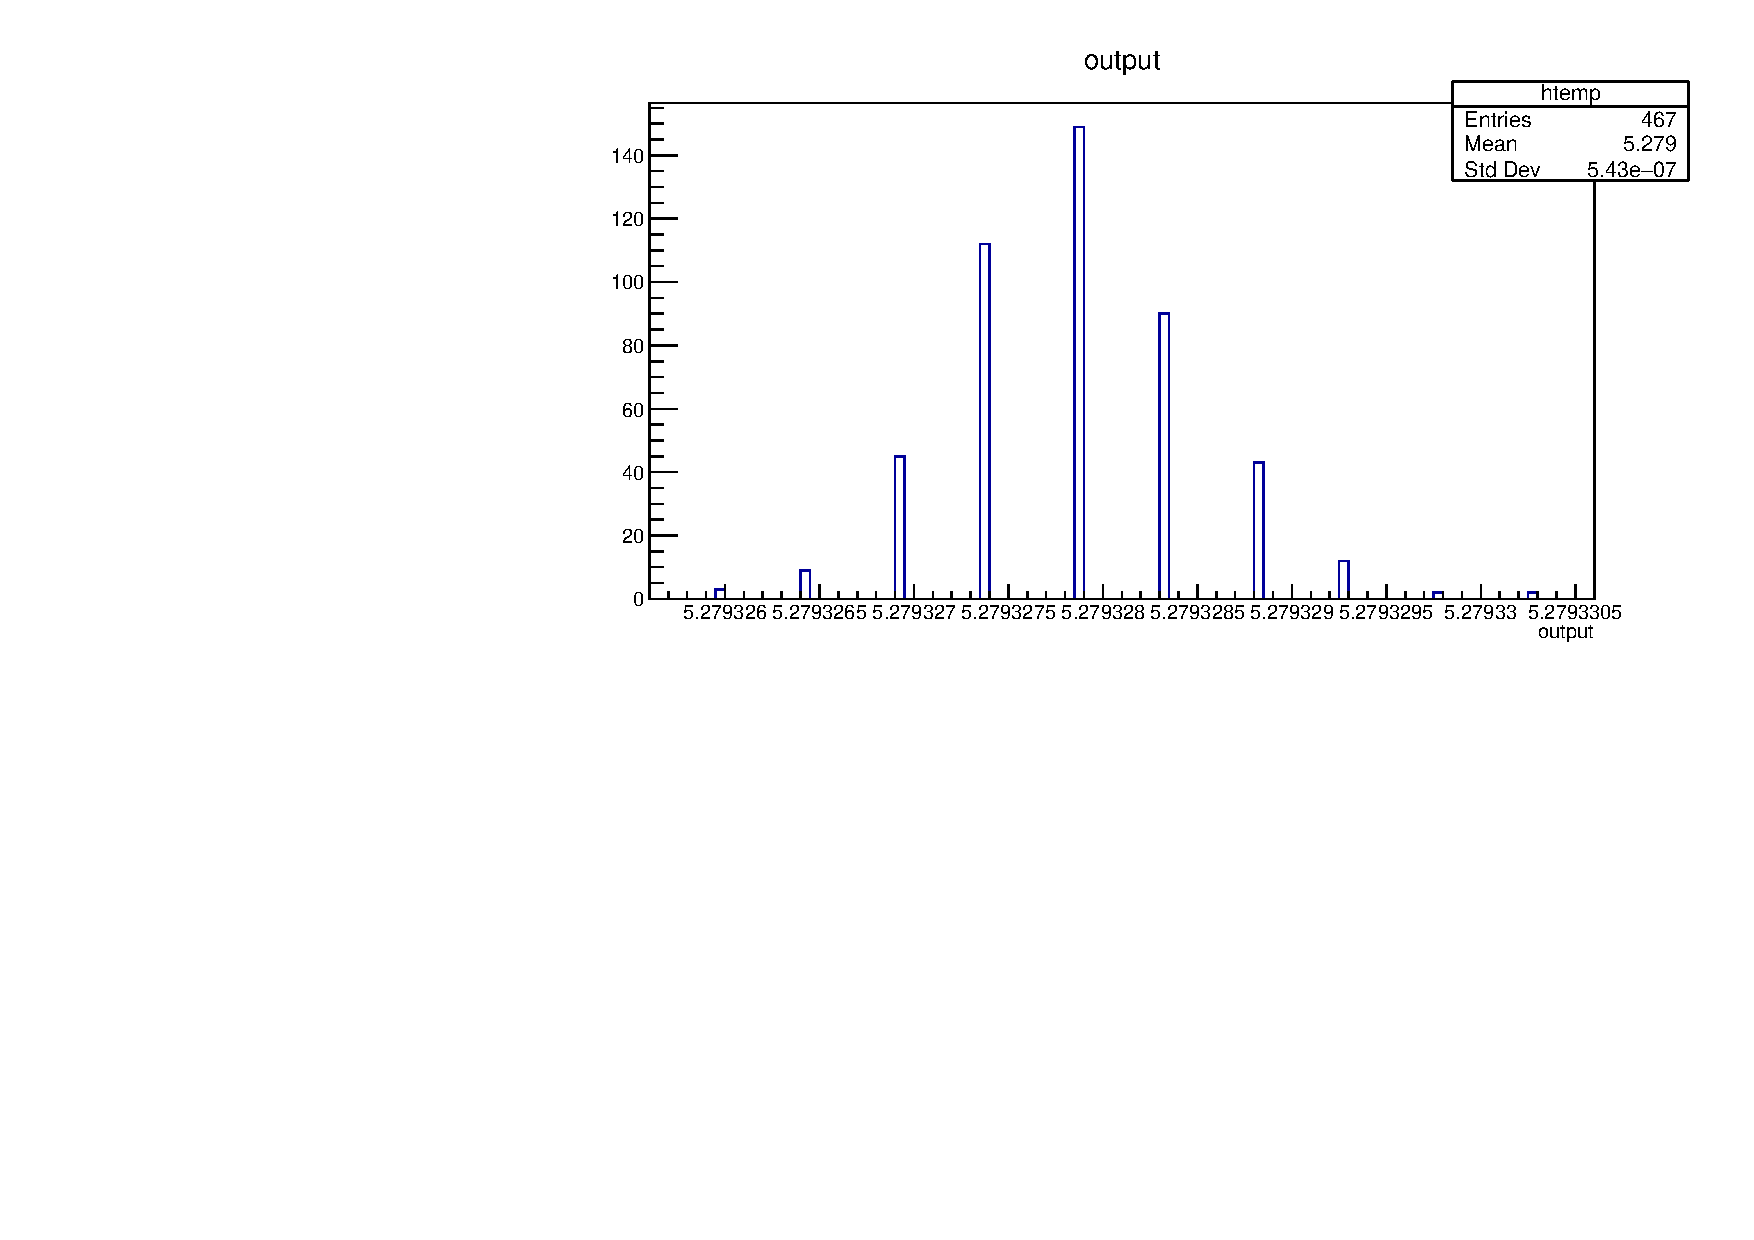
\includegraphics[width=0.5\linewidth]{figures/predPN2.pdf}
    \caption{PN2}
    \label{PN2}
\end{figure}
\begin{figure}[H]
    \centering
    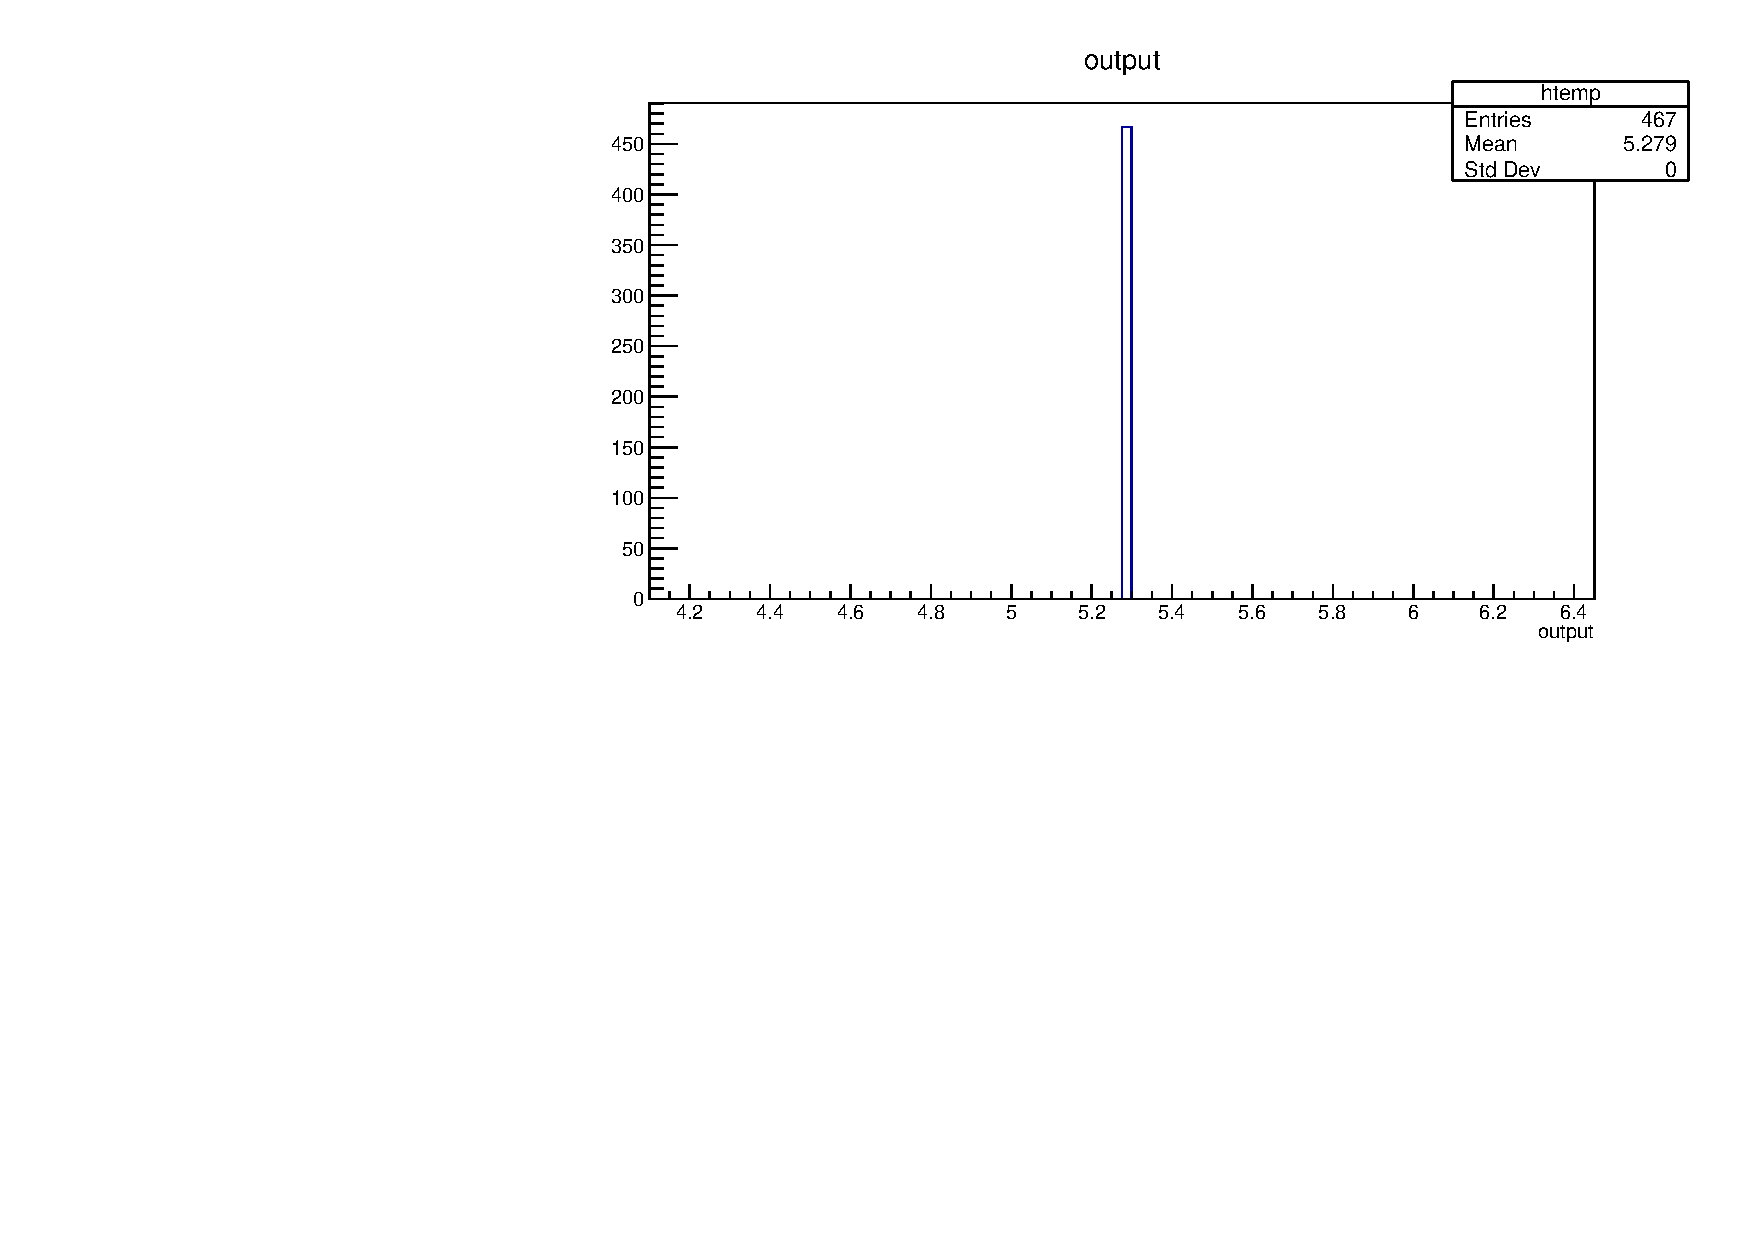
\includegraphics[width=0.5\linewidth]{figures/predPN3.pdf}
    \caption{PN3}
    \label{PN3}
\end{figure}
\begin{figure}[H]
    \centering
    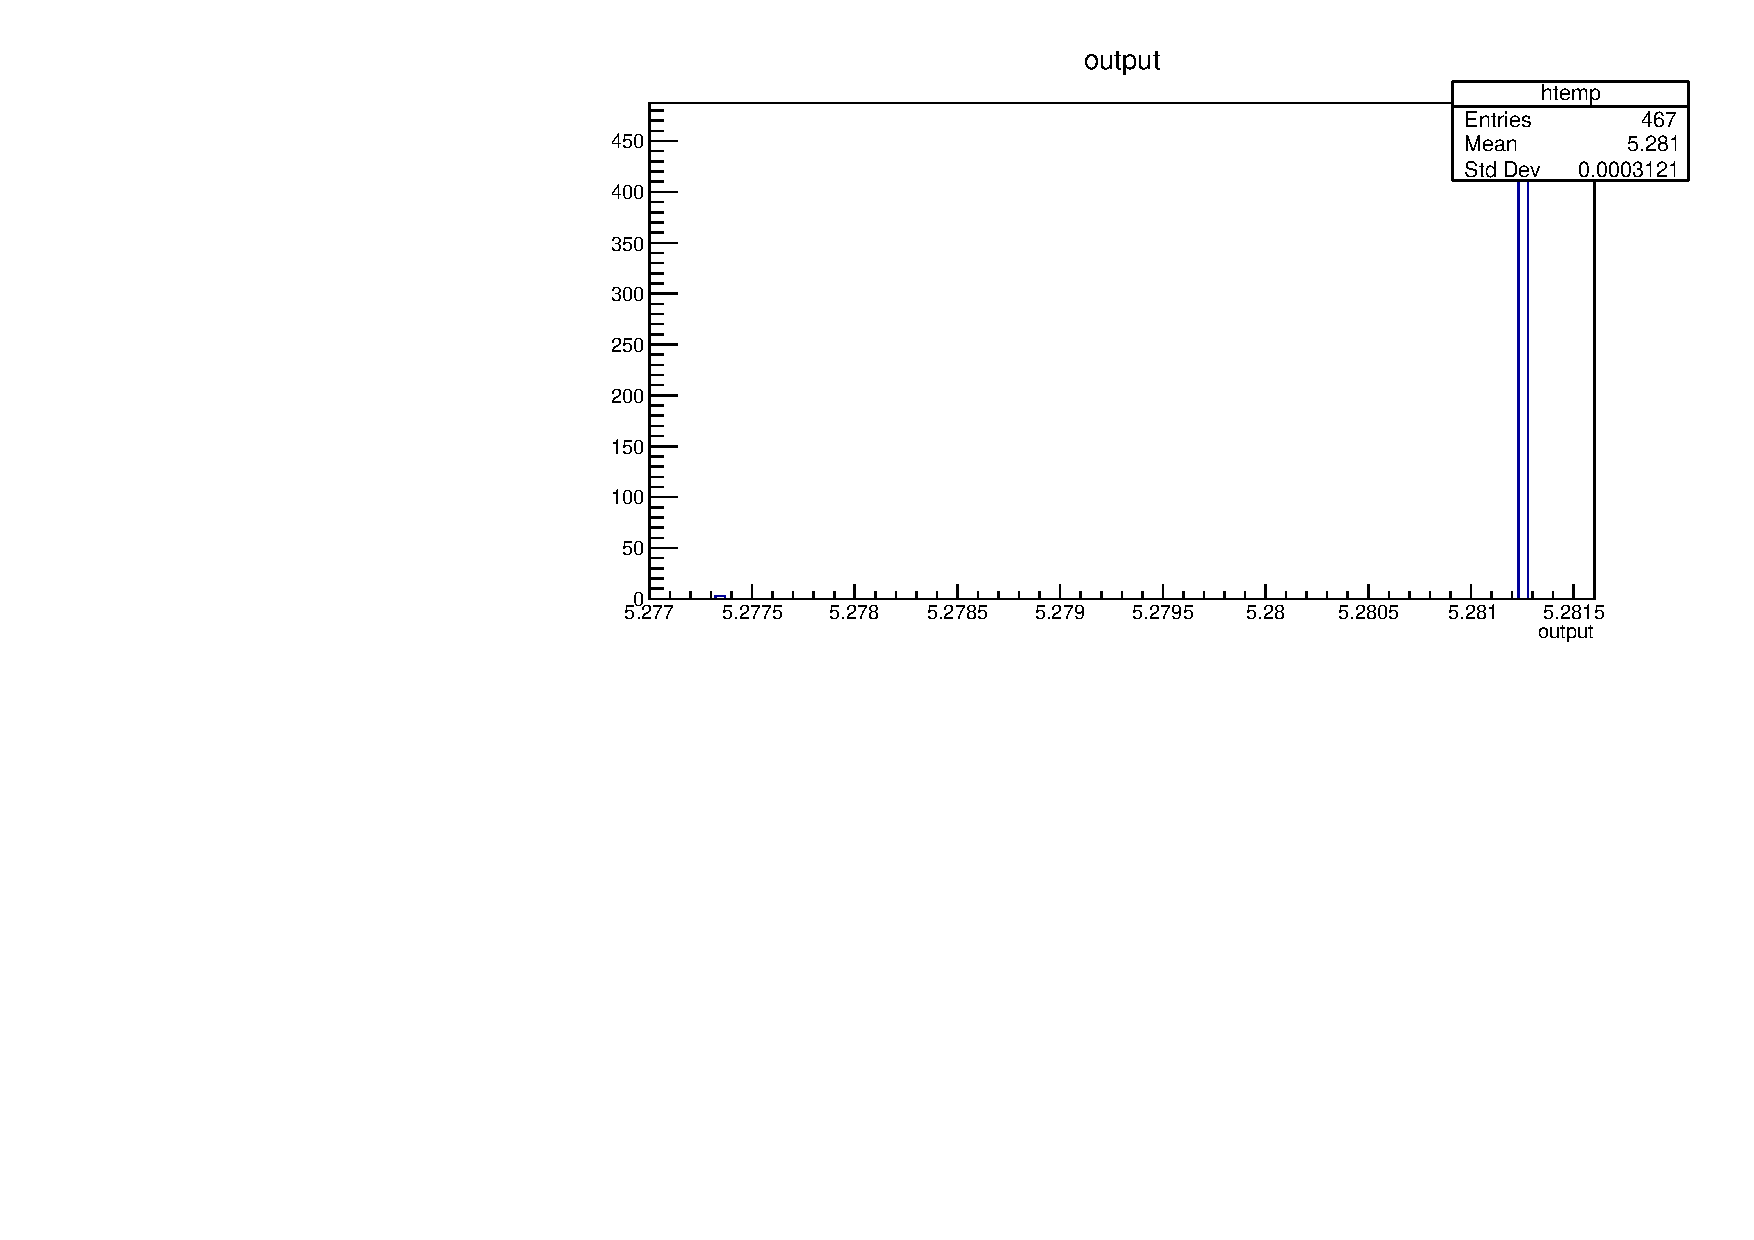
\includegraphics[width=0.5\linewidth]{figures/predParT1.pdf}
    \caption{ParT1}
    \label{ParT1}
\end{figure}
\begin{figure}[H]
    \centering
    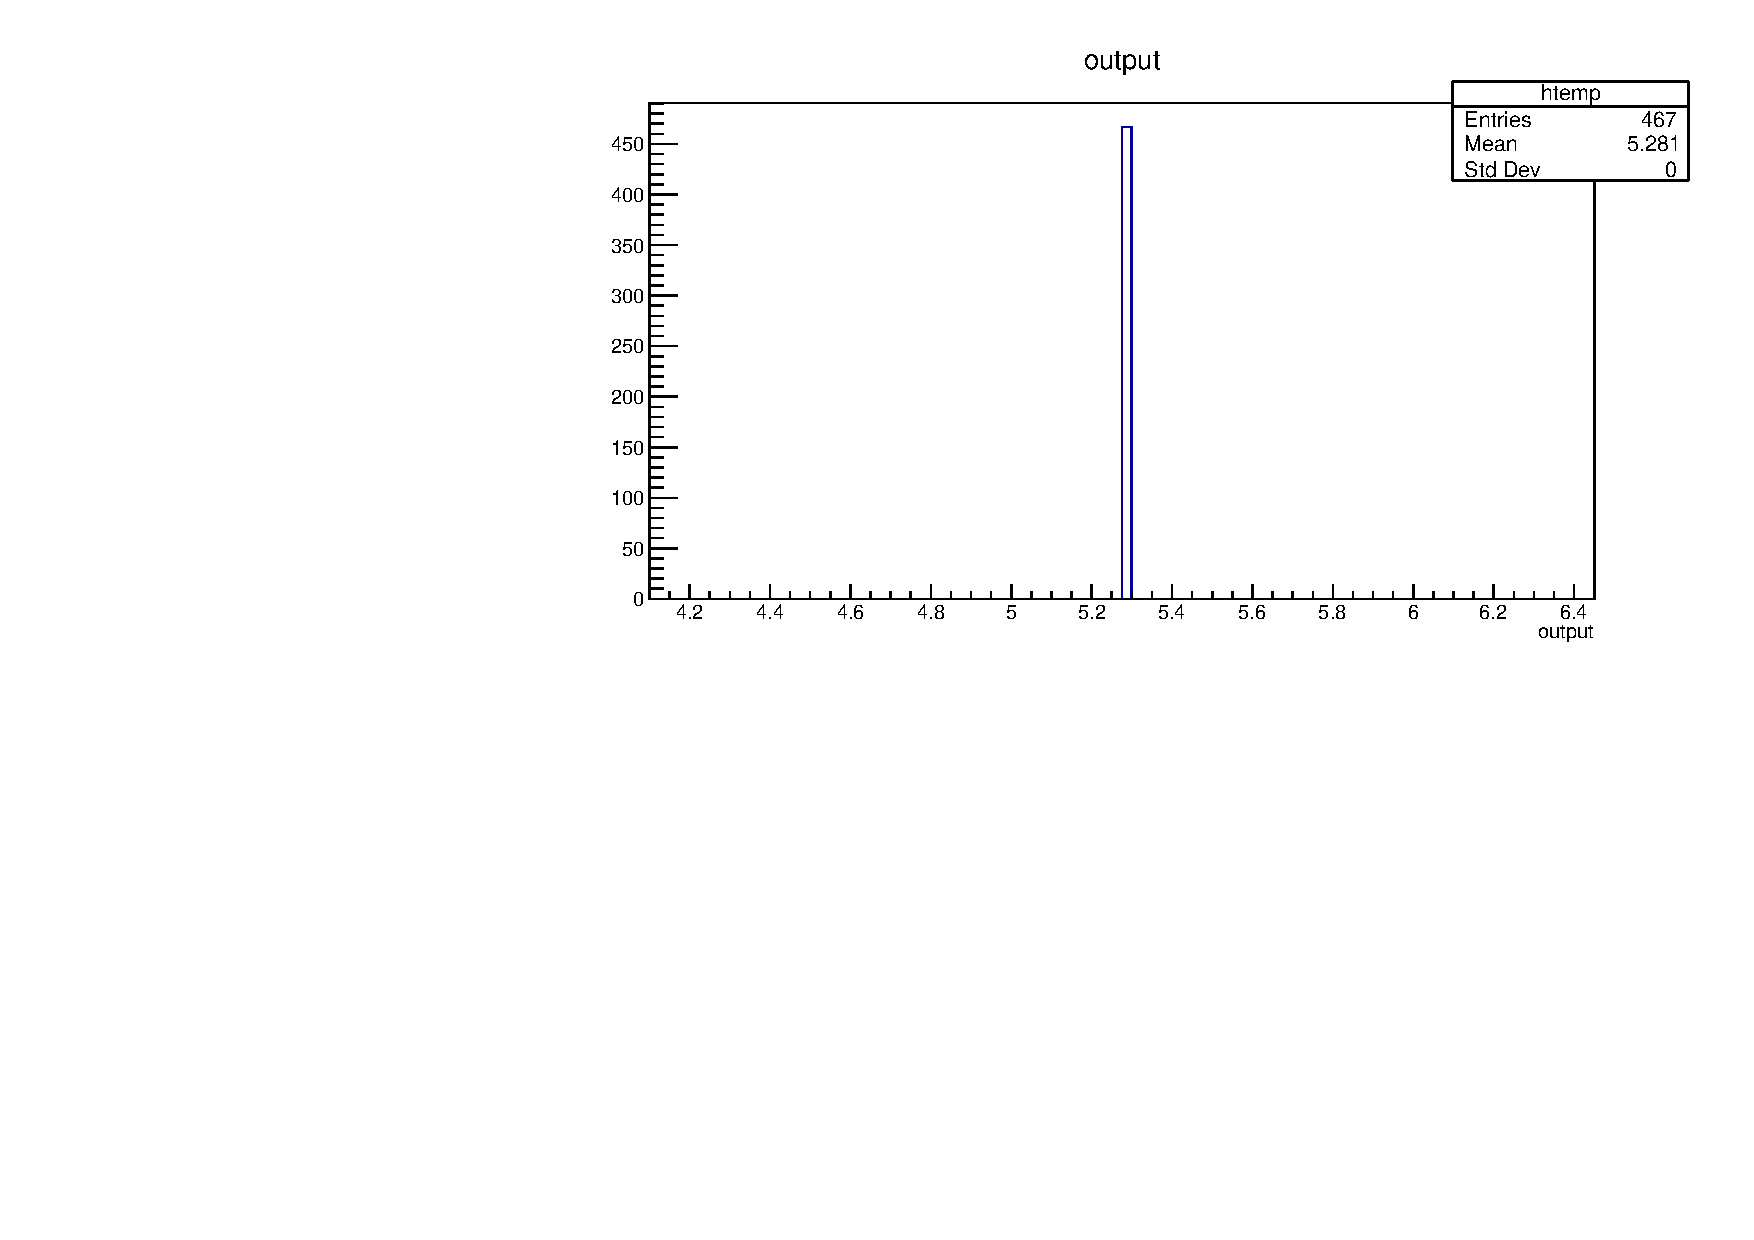
\includegraphics[width=0.5\linewidth]{figures/predParT2.pdf}
    \caption{ParT2}
    \label{ParT2}
\end{figure}

I found out that although the Particle Transformer seems to converge faster, but the prediction is biased, and the Particle Net can give a close prediction after training through $200$ epoches.
Next step is to increase the size of the data.
One can try to think about add some event shape variables that may be useful for training and identification.

\section{Theoretical Background: Event Generator}
This neural network is designed to reconstruct the mass of \(B^{+}\) meson from its final states.
The decay event we simulate is not the direct \(B^{+}\) meson decay, but \( \Upsilon ( 4S ) \) decay to \( B^{\pm} \) pair.
Now, we first analyze the structure of this event and the suitable event shape variables for its geometry.

Here we briefly record the final states of \(B^{ + }\) and \(B^{ - }\) decay.
A \(B^{ + }\) meson can decay into several gamma rays and pions; while a \(B^{ - }\) meson can decay into gamma rays, muons, pions, and muon neutrino.
We can consider that several particles are not detected by the physical detector, like neutrino.

Sometimes the simulation of \( Upsilon ( 4S ) \) decays into \( B^0 \) and \( \bar{ B^0 } \) pair.
\end{document}